\documentclass[autodetect-engine,twocolumn]{jsarticle}

\newif\ifuptexmode
\makeatletter
\if@jsc@uplatex
 \uptexmodetrue
\else
 \uptexmodefalse
\fi

\usepackage[dvips]{graphicx}
\begin{document}
\parindent0mm

dviware: dvips

\ifuptexmode
engine: upLaTeX
\typeout{### engine: upLaTeX ###}
\else
engine: pLaTeX
\typeout{### engine: pLaTeX ###}
\fi

inner-code: %
\ifnum\jis"2121="3000 Unicode%
\else
 \ifnum\jis"2121="A1A1
  EUC%
 \else
  SJIS%
\fi
\fi
\\

図のテスト。

go000.eps:\\
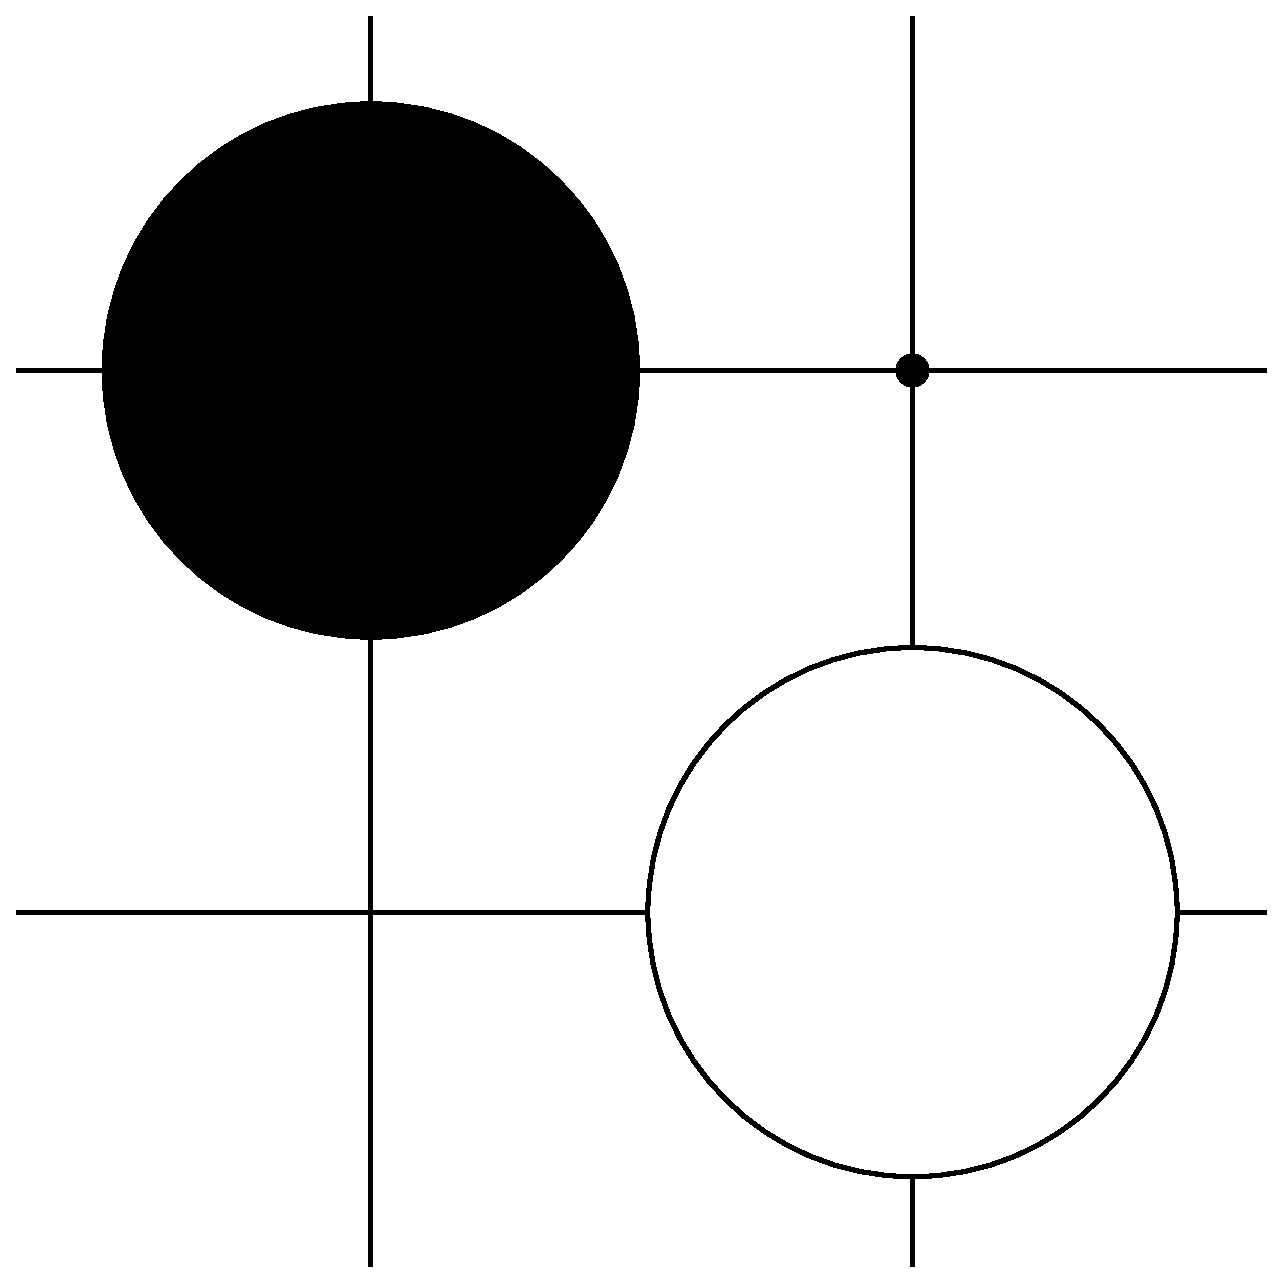
\includegraphics[width=30mm]{figures/go000.eps}

go001囲碁\_芸能\_予定表.eps:\\ %  Shift\_JISのダメ文字を含む
\includegraphics[width=30mm]{figures/go001囲碁_芸能_予定表.eps}

長いファイル名:\\
\includegraphics[width=30mm]{figures/go002囲碁爛柯坐隠手談烏鷺方円囲碁爛柯坐隠手談烏鷺方円囲碁爛柯坐隠手談烏鷺方円囲碁爛柯坐隠手談烏鷺方円囲碁爛柯坐隠手談烏鷺方円囲碁爛柯坐隠手談烏鷺方円.eps}

\end{document}

